

\documentclass[12pt]{article}
\usepackage{graphicx}
\usepackage{amsmath}
\usepackage{listings}
\usepackage{color}
\usepackage[section]{placeins} %this stops the figures from showing up in wrong section

\definecolor{dkgreen}{rgb}{0,0.6,0}
\definecolor{dkblue}{rgb}{0,0.0,0.6}
\definecolor{dkred}{rgb}{0.9,0.0,0.1}


\begin{document}

\lstset{language=Fortran,tabsize=4,numbers=left,numberstyle=\tiny,basicstyle=\ttfamily\small\color{dkblue},stringstyle=\ttfamily\color{blue},keywordstyle=\rmfamily\color{dkred}\bfseries\emph,backgroundcolor=\color{white},commentstyle=\color{dkgreen}}




\title{Physics 562 - Computational Physics\\[.5cm]
Assignment 1: Fourier's law}
\author{Josh Fernandes\\
Department of Physics \& Astronomy\\
California State University Long Beach}
\date{\today}

  
\maketitle



\begin{abstract}
For this assignments we are practicing some pasic coding concepts in Fortran as well as \LaTeX~  We are given Fourier's law to paramaterize and then graph the outcome $\Theta$. We then practice basic unix command to pipe our data in to a data file and graph using PlotPublish. We then needed to publish our results in /LaTex~and learn to use Makefiles. 
\end{abstract}

\section{Introduction}\label{s:intro}

This is the first assignment for the class. The purpose of the assignment is to familiarize ourselves with Fortran,Make file, and LaTeX notation. Fortran dates back to 1953, but it has been updated nine times since it's release. This class focuses on Fortran95, but there are more recent versions of Fortran with another update coming in 2015. This paper solves a scattering coefficient equation for several values of $\Gamma$. The results are plotted on the same graph, so the effect of $\Gamma$ on the shape of the curve can be determined. 



\section{The Fortran95 code}

The fortran code solves a one dimensional scattering equation. There is a transmission coefficient that represents a probability of a particle being transmitted. It ranges from 0 to 1. It is centered at some Energy ${E}_{0}$ . The function also depends on a constant denoted by $\Gamma$. The formula is 

\begin{gather}
T = \frac{\frac{1}{4}\Gamma^2}{(E-E_0)^2 + \frac{1}{4}\Gamma^2}.
\end{gather}

The Makefile in Listing \ \ref{makefile} describes the structure of the code. The codes in {\tt OBJS1} are 
compiled together. The {\tt .o} files were created from the {\tt .f95} file by using the {\tt F95} command
with flags {\tt F95FLAGS}. In building the executable code {\tt LDFLAGS} were used, which contains 
the {\tt LIB} library. These {\tt LDFLAGS} are optimal for Intel Core2 architecture and uses the 
Apple's {\tt vecLib} library from Xcode. By typing {\tt make} we can produce the executable file.





\begin{lstlisting}[frame=single,caption={Typical {\tt Makefile}},label=makefile]

OBJS = numtype.o scattering.o 

PROG = scattering

F95 = gfortran

F95FLAGS = -O3 -funroll-loops -fexternal-blas

LIBS = -framework vecLib

LDFLAGS = $(LIBS)

all: $(PROG) 

$(PROG): $(OBJS)
	$(F95) $(LDFLAGS) -o $@ $(OBJS) 

clean:
	rm -f $(PROG) *.{o,mod}

.SUFFIXES: $(SUFFIXES) .f95

.f95.o:
	$(F95) $(F95FLAGS) -c $<

\end{lstlisting}

The Fortran95 code is shown below. The precision is defined in the Module {\tt NumType}. The constants parameters are defined in Module {\tt setup}. The implicit none statement ensures that all the variables has to be defined. {\tt do while-end do} is used to increase the value of E while also calculating T for the four different $\Gamma$ values. 


\begin{lstlisting}[frame=single,caption={Module {\tt NumType}},label=module]

module NumType

	save
	integer, parameter :: dp = kind(1.d0)
	real(dp), parameter :: pi = 4*atan(1._dp)
	complex(dp), parameter :: iic = (0._dp,1._dp)
	
end module NumType

\end{lstlisting}


\begin{lstlisting}[frame=single,caption={The {\tt scattering.f95}},label=scattering95]


module setup

	use NumType
	implicit none
	real(dp) :: E, dE, E0, gamma(4)
	REAL, DIMENSION(:, :), ALLOCATABLE :: T
	integer :: i, j, N, M, DeAllocateStatus,
	AllocateStatus, Emax
	

end module setup

program scattering_path

	use setup
	implicit none
	
	gamma  = (/ 1.0, 0.5, 0.1, 0.01/) 

	E = 0._dp
	dE = 0.01_dp
	Emax = 10_dp

	E0 = 5_dp	
	j = 0._dp		

	N = size(gamma)
	M = (Emax/dE)+1

	ALLOCATE ( T(N, M), STAT = AllocateStatus)
	IF (AllocateStatus /= 0) STOP 
	"*** Not enough memory ***"
		
	do while (E < Emax)
		j = j + 1
		do i=1,4
			T(i,j) = (.25*(gamma(i)**2))/((E-E0)**2 + 
			.25*(gamma(i)**2))
		end do
		print *, E, T(1,j), T(2,j), T(3,j), T(4,j)
		E = E + DE
	end do 
		
	DEALLOCATE (T, STAT = DeAllocateStatus)
end program scattering_path

\end{lstlisting}


The code is run by typing {\tt ./scattering}. The results are printed on the screen, or the data can redirect to the file {\tt 1} by typing {\tt ./scattering > 1}. The {\tt Plot} provides the picture in Fig.\ \ref{linearscattering} and Fig.\ \ref{logscattering}. 


\begin{figure}[!htb]
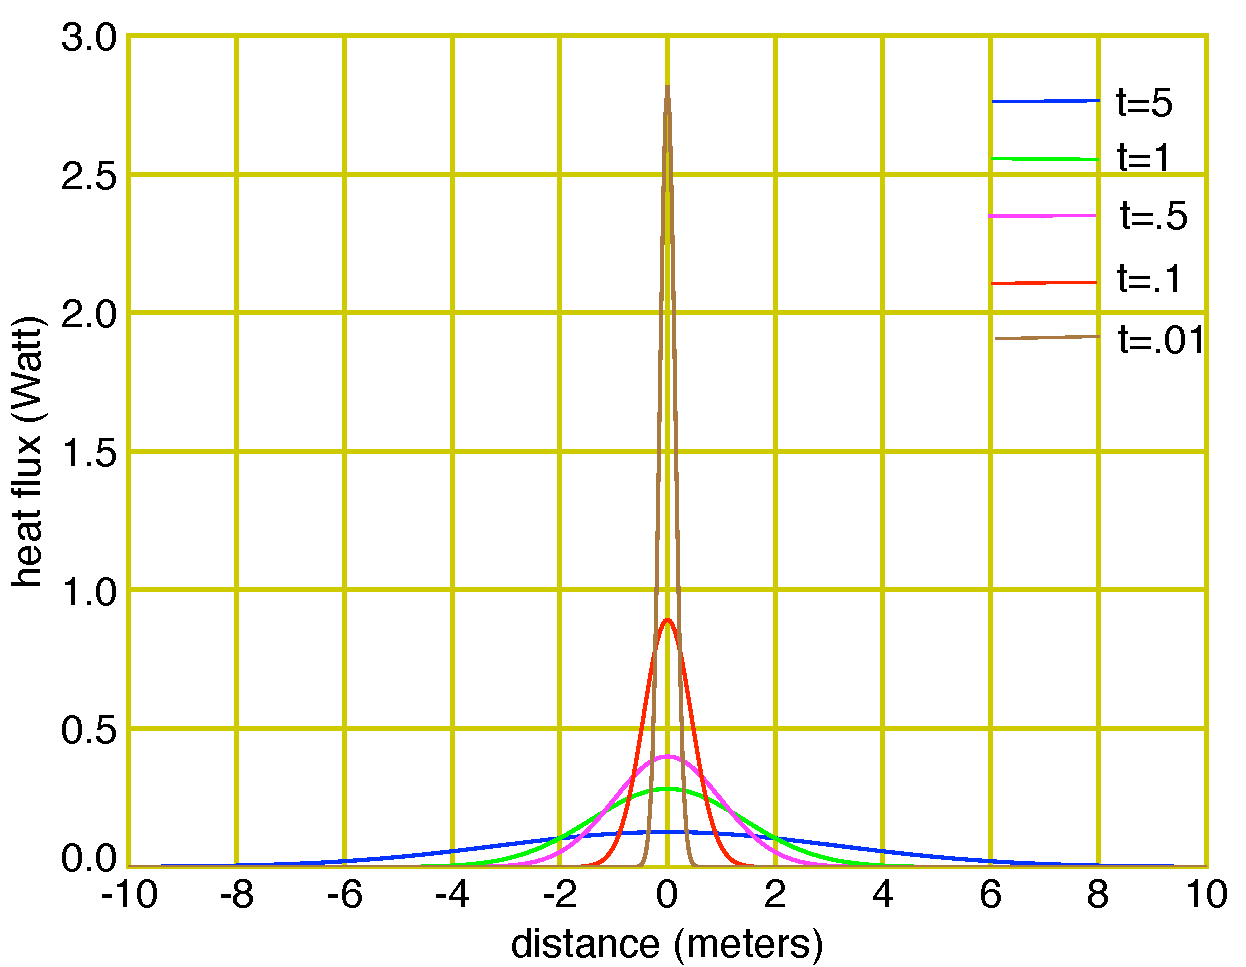
\includegraphics[width=1.\textwidth]{stufflinear.pdf}
\caption{Results of the {\tt heat.f95} code plotted on a linear scale. }
\label{linearscattering}
\end{figure}

\begin{figure}[!htb]
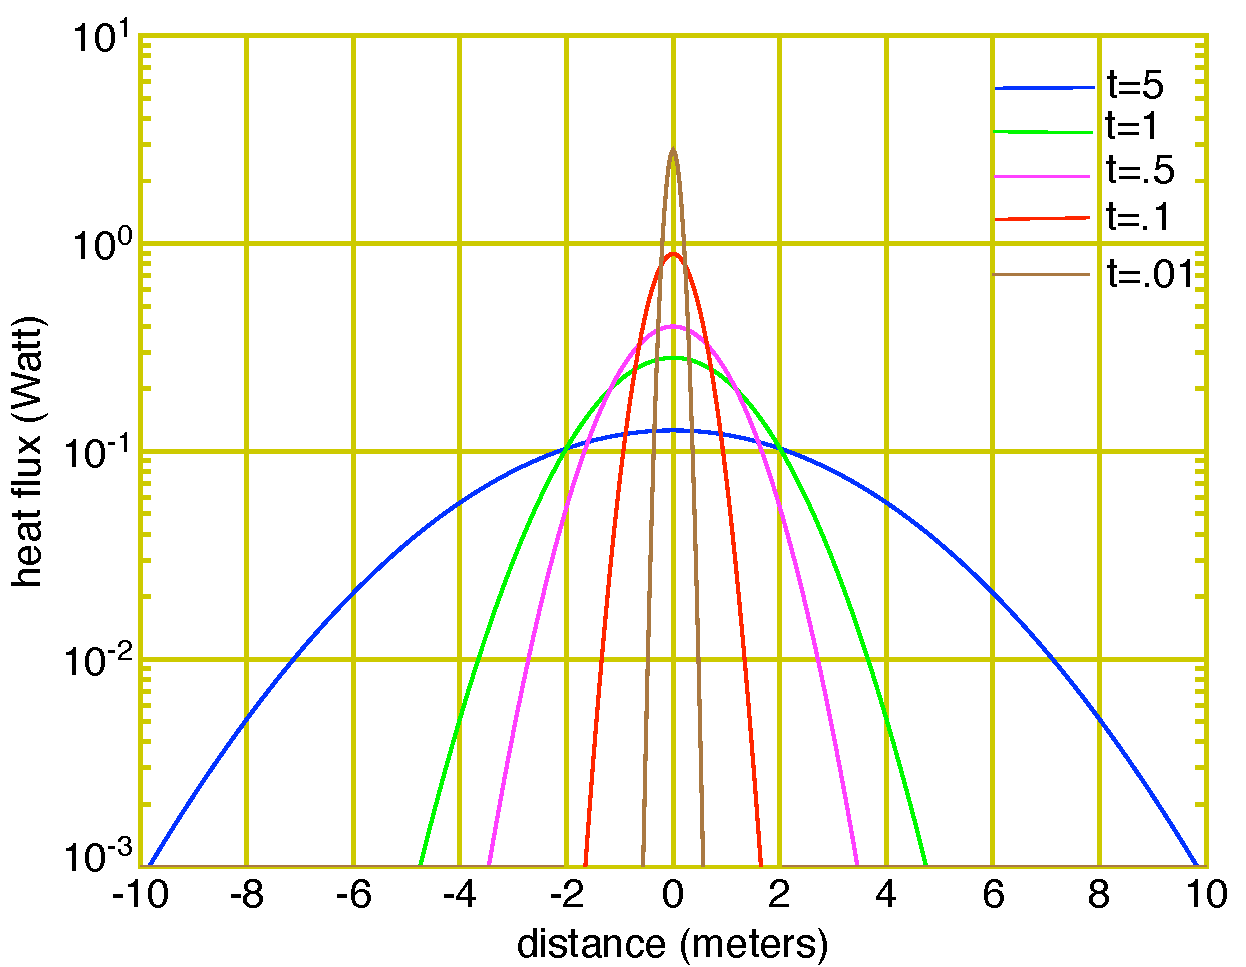
\includegraphics[width=1.\textwidth]{stufflog.pdf}
\caption{Results of the {\tt heat.f95} code plotted on a log scale. }
\label{logscattering}
\end{figure}





\section{Summary and conclusions}

The first Fortran95 code \cite{metcalf} for the class was written. The transmission coefficient as a function of E with four different $\Gamma$ values was plotted. The numerical results agree with our prior knowledge and expectations.

\begin{thebibliography}{}


\bibitem{metcalf} M.\ Metcalf, J.\ Reid and M.\ Cohen, {\it Fortran 95/2003 explained}. Oxford University Press, 2004.
 

\end{thebibliography}




\end{document}
